\documentclass[12pt, a4paper]{article}
\usepackage{../notesheets}

%%%%%%%%%%%%%%%%%%%%%%%%%%%%%%%%%%%%%%%%%%%%%%%%%%
\author{Math 1210}
\title{Notesheet. Section 4.2: Applications of the Second Derivative}
\date{}

\begin{document}
\maketitle
\nameline
%%%%%%%%%%%%%%%%%%%%%%%%%%%%%%%%%%%%%%%%%%%%%%%%%%
\begin{defi}
  Let a function \(f\) be differentiable on an interval
  \((a,b)\). Then,
  \begin{enumerate}
  \item \(f\) is \de{concave upward} on \((a,b)\) if
  \item \(f\) is \de{concave downward} on \((a,b)\) if
  \end{enumerate}
\end{defi}
\vspace{-0.5in}
\begin{ex}
  Where is the following graph concave upwards and where is it concave
  downwards?\\
  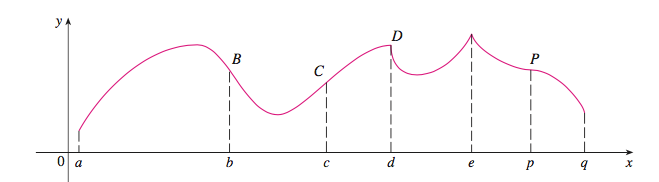
\includegraphics[scale=0.5]{images/concavity-example}
\end{ex}
\vspace{-2.2in}
\begin{ex}
  Consider the function \(f(x) = x^3\). Where is \(f\) concave upward
  and where is it concave downward? What can we say about \(f''(x)\)
  on these intervals?
\end{ex}
\begin{thrm}
  Let \(f\) be twice differentiable on an interval \((a,b)\). Then,
  \begin{enumerate}
  \item If \(f''(x) > 0\) for each value of \(x\) in \((a,b)\), then
  \item If \(f''(x) < 0\) for each value of \(x\) in \((a,b)\), then
  \end{enumerate}
\end{thrm}
\vspace{-0.5in}
\begin{defi}
  A \de{point of inflection} \((a,f(a))\) on a graph of a function \(f\) is
\end{defi}
\begin{ex}
  What is the second derivative of \(f(x) = x^3\) at the point(s) of
  inflection? What is the second derivative at the point(s) of
  inflection of \[
    g(x) =
    \begin{cases}
      \frac{1}{x} & x \neq 0\\
      0 & x = 0
    \end{cases}
  \]
  Finally, does \(h(x) = x^4\) have any inflection points?
\end{ex}
\begin{thrm}
  If \((a,f(a))\) is an inflection point for the graph of \(f\),
  then \(f''(a) = 0\) \textbf{or \(f''(a)\) does not exist.}
\end{thrm}
\vspace{-1in}
\begin{ex}
  Consider the function \(f(x) = x^4-4x^3\). Where is \(f\) concave up
  and concave down? Where are its points of inflection? Find the
  points where \(f'(x) = 0\) and evaluate the second derivative of
  \(f\) at these points.
\end{ex}
\begin{thrm}
  Let \(f\) be a twice differentiable function. Then, if \(f'(c) = 0\)
  and
  \begin{enumerate}
  \item \(f''(c) < 0\), then
  \item \(f''(c) > 0\), then
  \item \(f''(c) = 0\), then
  \end{enumerate}
\end{thrm}
%%%%%%%%%%%%%%%%%%%%%%%%%%%%%%%%%%%%%%%%%%%%%%%%%%
\end{document}
